\section{The audited framework and what its split implies}\label{sec:framework}

\subsection{The release}

CCMusic \citep{zhou2025ccmusic} is a Chinese-music resource whose associated article documents
six datasets, from instrumental technique corpora to popular-song excerpts, and evaluates all six
through one framework. The release we audited is larger than the article: it comprises thirteen
library directories published under the same ModelScope organisation, of which the six datasets
described in the article are a subset. Each library ships chroma, CQT and MEL features computed
from the audio, stored as one image per short-time window; the article notes that the MEL
spectrogram is provided alongside the audio for visualisation. The evaluation framework pools
datasets that share a task and trains a common classifier per task. We checked the version of
record in TISMIR 8(1), pp. 22--38 (2025), against the arXiv release and against the archives we
downloaded on 2 November 2026. On printed p. 26 the article states, for CTIS, that the dataset
was randomly split into training, validation and testing sets at a ratio of 8:1:1 after
2-second segmentation, at 43{,}054 clips, without naming the split unit; p. 28 gives a
recording-level 79:10:10 split for Guzheng Tech99, p. 29 a 6:2:2 ratio for ErhuPT without naming
the unit, and the remaining collections are given only an 8:1:1 ratio. No recording-group
constraint is attached to the stated evaluation protocol. This supports auditing the slice-level
interpretation where the statement names no unit, but does not recover the original authors'
actual split files.

Two properties of the release shape the audit. First, the feature images are the unit of
analysis: for the MEL family, each image is a 496$\times$369 JPEG whose file name encodes the
recording identifier and the window index. What ships beside the images also differs in what can be checked: all five libraries release
source audio, but only in CTIS do the audio file names map unambiguously onto the evaluation
recording identifiers, so the five libraries in Table~\ref{tab:panels} are not equally checkable
against the audio. Second, the
same recording contributes many images --- between 8.7 and 48.9 per recording across the five
libraries we use, as Table~\ref{tab:panels} lists --- so the number of images per recording is large
enough for a slice-level split to place many siblings of every test recording in training.

\subsection{The split statement}

The framework states that each dataset is ``randomly split \ldots at a ratio of 8:1:1''. The
statement does not name the unit of splitting, and the released files support a slice-level
reading: a split over image files. We verified that the article states no grouping constraint
in the stated evaluation description --- by recording, song, performer or album. Under the slice-level reading almost every test slice has siblings in training. If the
80/10/10 split is drawn independently per slice, then conditional on one slice of a recording
sitting in the sealed panel, the probability that at least one of its remaining $K-1$ slices
lands in training is $1-0.2^{K-1}$, since each sibling avoids the 80\% training share with
probability 0.2. It is 0.99999744 at $K=9$ and exceeds 0.999999999 at $K=14$ and $K=21$.
This is an independent-allocation calculation, not an exact formula for a fixed-size,
without-replacement partition. The
unconditional probability that a recording of $K$ slices contributes at least one training slice
is $1-0.2^{K}$. Figure~\ref{fig:units} contrasts the two units on one recording in its top two rows, and then
shows how the pool moves between panels in its bottom two rows.

\begin{figure}[!t]
\centering
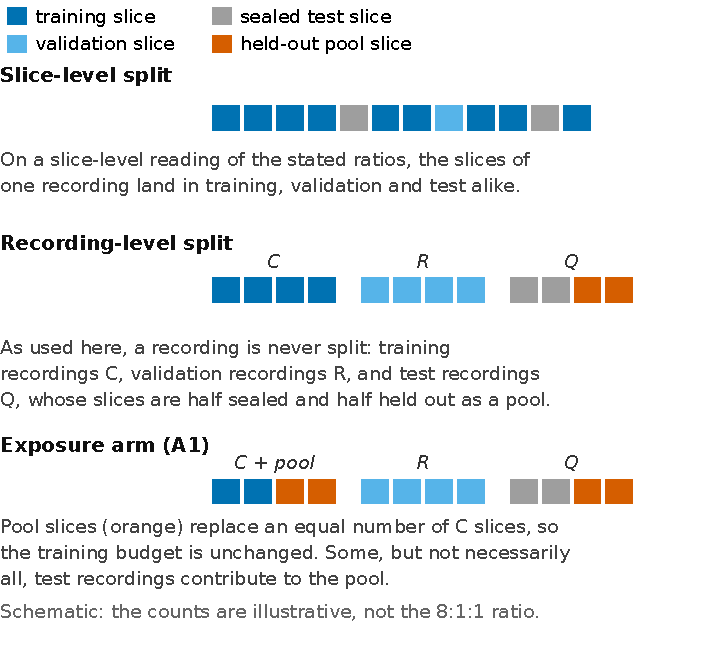
\includegraphics[width=\linewidth]{../figures/fig1_split_units.pdf}
\caption{Split units and the exposure intervention (schematic, not an exact 8:1:1 allocation).
Top: a slice-level partition can place siblings in training, validation and test. Middle: the
recording-disjoint allocation assigns training recordings to C, validation recordings to R,
and test recordings to Q; Q is then divided into sealed $Q_{\mathrm{test}}$ and
held-out $Q_{\mathrm{pool}}$ slices. Bottom: A1 replaces C slices with
$Q_{\mathrm{pool}}$, while $Q_{\mathrm{test}}$ remains sealed.}
\label{fig:units}
\end{figure}

We treat this as a specification question rather than an accusation. A database paper can leave an evaluation detail underspecified without establishing that its
implemented split was defective. We therefore distinguish the stated recipe, our slice-level
reconstruction, and the unavailable original split files. What the audit adds is the size of the gap between the protocol as stated and the protocol a
reader would need to interpret the number as generalisation to unseen music. The exposure
distribution, the capacity calculation and the four-arm contrast support that gap jointly; A2
contributes only a slice-level approximation.

\subsection{Terms}

We use \emph{recording} for the unit that a split should respect, meaning one performance or one
file in the source collection, \emph{slice} for one released feature image, $\bar K$ for the mean
number of slices per recording in a library, and \emph{homologous content} for the slices of a
recording whose other slices are in the test set. The implemented Q pool can also contain
recordings without test slices because grouped allocations need not put every recording on both
sides; A1 injects the full pool, not solely the homologous subset. A recording-level split is one in which all
slices of a recording fall on the same side of the partition.
